\documentclass[11pt]{article}
\usepackage{worksheet_style}

% ---- Toggle: uncomment for filled version ----
%\worksheetfilledtrue
\begin{document}
\worksheetheader{17}{Double Integrals over General Regions}

\begin{background}
Last time we integrated over rectangles. Most regions of interest---disks, triangles, regions between curves---aren't rectangular. Today we handle general regions using Type I and Type II setups, and introduce polar coordinates for circular symmetry. The Gaussian integral, which cannot be evaluated by single-variable methods, yields beautifully to the polar approach.
\end{background}

%=============================================================
\wsection{Warm-Up: Double Integral over a Rectangle}

Evaluate $\ds\int_0^2\int_1^3 (3xy^2)\,dy\,dx$.

1. Inner integral ($y$): $\ds\int_1^3 3xy^2\,dy = \wbml{3x\left[\frac{y^3}{3}\right]_1^3 = x(27-1)=26x}$

2. Outer integral ($x$): $\ds\int_0^2 26x\,dx = \wbml{[13x^2]_0^2 = 52}$

3. Result: $\wbm{\boxed{52}}$

%=============================================================
\wsection{Type I Regions (Vertical Slicing)}

\begin{defbox}{Type I Region}
$R = \{(x,y) : a \le x \le b,\; g_1(x) \le y \le g_2(x)\}$
\[\iint_R f(x,y)\,dA = \wbml{\int_a^b \int_{g_1(x)}^{g_2(x)} f(x,y)\,dy\,dx}\]
-- Integrate $y$ first (inner), then $x$ (outer)

-- Think: vertical lines sweep left to right across the region
\end{defbox}

%=============================================================
\wsection{Type II Regions (Horizontal Slicing)}

\begin{defbox}{Type II Region}
$R = \{(x,y) : c \le y \le d,\; h_1(y) \le x \le h_2(y)\}$
\[\iint_R f(x,y)\,dA = \wbml{\int_c^d \int_{h_1(y)}^{h_2(y)} f(x,y)\,dx\,dy}\]
-- Integrate $x$ first (inner), then $y$ (outer)

-- Think: horizontal lines sweep bottom to top across the region
\end{defbox}

\wsubsection{How to Classify a Region}

\begin{itemize}[nosep, leftmargin=*]
  \item Sketch the region and find all intersection points
  \item Type I -- can every vertical line ($x = c$) enter through one curve and exit through one curve?
  \item Type II -- can every horizontal line ($y = c$) enter through one curve and exit through one curve?
  \item Some regions work as both; pick whichever is simpler
  \item If neither works cleanly, \textbf{split} the region
\end{itemize}

\begin{center}
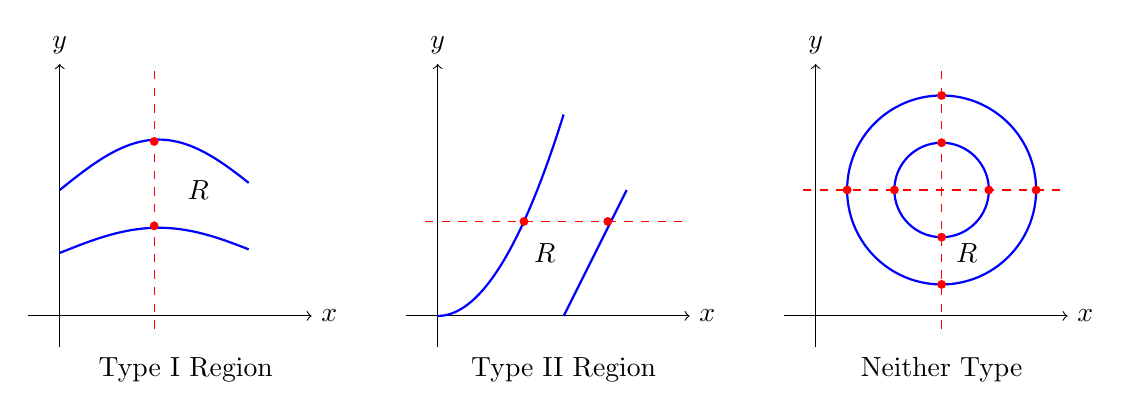
\begin{tikzpicture}[scale=0.8]
    \begin{scope}[local bounding box=plot1]
        \draw[->] (-0.5,0) -- (4,0) node[right] {$x$};
        \draw[->] (0,-0.5) -- (0,4) node[above] {$y$};
        \draw[thick, blue] plot[smooth, domain=0:3] (\x, {2 + 0.8*sin(\x r)});
        \draw[thick, blue] plot[smooth, domain=0:3] (\x, {1 + 0.4*sin(\x r)});
        \draw[dashed, red] (1.5,-0.2) -- (1.5,4);
        \fill[red] (1.5,2.77) circle (2pt);
        \fill[red] (1.5,1.43) circle (2pt);
        \node at (2.2,2) {$R$};
        \node[below] at (2,-0.5) {Type I Region};
    \end{scope}
    \begin{scope}[xshift=6cm, local bounding box=plot2]
        \draw[->] (-0.5,0) -- (4,0) node[right] {$x$};
        \draw[->] (0,-0.5) -- (0,4) node[above] {$y$};
        \draw[thick, blue] plot[domain=0:2, samples=50] (\x, {0.8*\x*\x});
        \draw[thick, blue] plot[domain=0:2, samples=50] ({2 + 0.5*\x}, \x);
        \draw[dashed, red] (-0.2,1.5) -- (4,1.5);
        \fill[red] (1.37,1.5) circle (2pt);
        \fill[red] (2.7,1.5) circle (2pt);
        \node at (1.7,1) {$R$};
        \node[below] at (2,-0.5) {Type II Region};
    \end{scope}
    \begin{scope}[xshift=12cm, local bounding box=plot3]
        \draw[->] (-0.5,0) -- (4,0) node[right] {$x$};
        \draw[->] (0,-0.5) -- (0,4) node[above] {$y$};
        \draw[thick, blue] (2,2) circle (1.5);
        \draw[thick, blue] (2,2) circle (0.75);
        \draw[dashed, red] (2,-0.2) -- (2,4);
        \draw[dashed, red] (-0.2,2) -- (4,2);
        \foreach \y in {0.5,1.25,2.75,3.5} { \fill[red] (2,\y) circle (2pt); }
        \foreach \x in {0.5,1.25,2.75,3.5} { \fill[red] (\x,2) circle (2pt); }
        \node at (2.4,1) {$R$};
        \node[below] at (2,-0.5) {Neither Type};
    \end{scope}
\end{tikzpicture}\\
{\small A Type I region is bounded above and below by functions of $x$ — every vertical line (red) hits the boundary exactly twice. Type II is analogous with horizontal lines. An annulus is \emph{neither}: both horizontal and vertical slice lines can cross the boundary four times, so it must be split.}
\end{center}

%=============================================================
\wsection{Examples}

\begin{example}[Type I: Region Between Two Parabolas]
Evaluate $\ds\iint_R (x+2y)\,dA$ where $R$ is bounded by $y = x^2$ and $y = 2 - x^2$.

\wbbox{
1. \textbf{Sketch and intersections:} $x^2 = 2-x^2 \implies 2x^2 = 2 \implies x = \pm 1$.

\quad Lower curve: $y = x^2$. \quad Upper curve: $y = 2-x^2$.

2. \textbf{Set up (Type I):}
\[\int_{-1}^{1}\int_{x^2}^{2-x^2}(x+2y)\,dy\,dx\]

3. \textbf{Inner integral ($y$):}
$[xy + y^2]_{x^2}^{2-x^2} = x(2-x^2)+(2-x^2)^2 - x\cdot x^2 - x^4$

$= 2x - x^3 + 4 - 4x^2 + x^4 - x^3 - x^4 = 2x - 2x^3 - 4x^2 + 4$

4. \textbf{Outer integral ($x$):} Note $2x - 2x^3$ is odd on $[-1,1]$ so integrates to $0$.

$\int_{-1}^1(-4x^2+4)\,dx = 2\int_0^1(-4x^2+4)\,dx = 2\left[-\frac{4x^3}{3}+4x\right]_0^1 = 2\left(\frac{8}{3}\right)$

5. \textbf{Result:} $\boxed{\dfrac{16}{3}}$
}{6cm}
\end{example}

\begin{example}[Polar: Integral over a Disk]
Evaluate $\ds\iint_D (x^2+y^2)\,dA$ where $D$ is the disk $x^2 + y^2 \le 4$.

\wbbox{
1. \textbf{Convert to polar:} $x^2+y^2 = r^2$, $dA = r\,dr\,d\theta$.

\quad Disk: $0 \le r \le 2$, $0 \le \theta \le 2\pi$.

2. \textbf{Set up:}
$\ds\int_0^{2\pi}\int_0^2 r^2 \cdot r\,dr\,d\theta = \int_0^{2\pi}d\theta \cdot \int_0^2 r^3\,dr$

3. \textbf{Evaluate:}
$= 2\pi \cdot \left[\frac{r^4}{4}\right]_0^2 = 2\pi \cdot 4$

4. \textbf{Result:} $\boxed{8\pi}$
}{4cm}
\end{example}

%=============================================================
\wsection{Polar Coordinates for Double Integrals}

\begin{formulabox}{Double Integrals in Polar}
\[\iint_R f(x,y)\,dA = \int_\alpha^\beta \int_{r_1(\theta)}^{r_2(\theta)} f(r\cos\theta,\, r\sin\theta)\cdot r\,dr\,d\theta\]
-- The extra factor of $r$ comes from the area element: $dA = r\,dr\,d\theta$

-- Use polar when the region or integrand involves $x^2+y^2$, circles, or sectors
\end{formulabox}

\begin{example}[The Gaussian Integral ($I^2$ Trick)]
Evaluate $I = \ds\int_{-\infty}^{\infty} e^{-x^2}\,dx$.

\wbbox{
1. \textbf{Square the integral:}
$I^2 = \left(\int_{-\infty}^{\infty}e^{-x^2}\,dx\right)\left(\int_{-\infty}^{\infty}e^{-y^2}\,dy\right) = \iint_{\R^2} e^{-(x^2+y^2)}\,dA$

2. \textbf{Convert to polar:} $x^2+y^2 = r^2$, region is all of $\R^2$.
\[I^2 = \int_0^{2\pi}\int_0^{\infty} e^{-r^2}\cdot r\,dr\,d\theta\]

3. \textbf{Inner integral:} Let $u = -r^2$, $du = -2r\,dr$:
$\int_0^{\infty}r\,e^{-r^2}\,dr = \left[-\frac{1}{2}e^{-r^2}\right]_0^\infty = 0 - \left(-\frac{1}{2}\right) = \frac{1}{2}$

4. \textbf{Outer integral:} $I^2 = 2\pi \cdot \frac{1}{2} = \pi$

5. \textbf{Result:} $I = \boxed{\sqrt{\pi}}$

\medskip
\textit{This integral cannot be evaluated by single-variable techniques --- the $I^2$ trick with polar coordinates is essential.}
}{6cm}
\end{example}

%=============================================================
\wsection{Complex Regions (Splitting)}

When a region is neither purely Type I nor Type II -- \textbf{split} it:
\[\iint_R f\,dA = \iint_{R_1} f\,dA + \iint_{R_2} f\,dA\]
You can even use Cartesian for one piece and polar for another.

\begin{example}[Split Region: Cartesian + Polar]
Evaluate $\ds\iint_R (1+x^2+y^2)\,dA$ where $R$ is the region inside the square $[-1,1]\times[-1,1]$ but outside the unit disk $x^2+y^2 < 1$, combined with the upper half-disk $x^2+y^2\le 1$, $y\ge 0$.

\wbbox{
1. \textbf{Split:} Let $R_1$ = upper half-disk ($x^2+y^2 \le 1$, $y \ge 0$) and $R_2$ = square minus full disk (corners).

2. \textbf{$R_1$ in polar:} $0 \le r \le 1$, $0 \le \theta \le \pi$.
\[\iint_{R_1}(1+r^2)\cdot r\,dr\,d\theta = \int_0^\pi\int_0^1 (r+r^3)\,dr\,d\theta = \pi\left[\frac{r^2}{2}+\frac{r^4}{4}\right]_0^1 = \frac{3\pi}{4}\]

3. \textbf{$R_2$:} The corners of the square outside the disk can be set up as a Cartesian integral:
\[\iint_{\text{square}}(1+x^2+y^2)\,dA - \iint_{\text{disk}}(1+x^2+y^2)\,dA\]
Square integral: $\int_{-1}^1\int_{-1}^1(1+x^2+y^2)\,dy\,dx = \frac{20}{3}$.

Full disk integral (polar): $\int_0^{2\pi}\int_0^1(1+r^2)r\,dr\,d\theta = 2\pi\cdot\frac{3}{4} = \frac{3\pi}{2}$.

Corners: $\frac{20}{3} - \frac{3\pi}{2}$.

4. \textbf{Combine:} Total $= \frac{3\pi}{4} + \frac{20}{3} - \frac{3\pi}{2} = \frac{20}{3} - \frac{3\pi}{4}$

5. \textbf{Result:} $\boxed{\dfrac{20}{3} - \dfrac{3\pi}{4}}$
}{7cm}
\end{example}

%=============================================================

\begin{practice}

\prob Evaluate $\ds\int_0^1\int_0^x xy\,dy\,dx$.

\wans{\wbm{$1/8$}}

\vspace{3cm}

\prob Evaluate $\ds\iint_R xy\,dA$ where $R$ is bounded by $y = 0$, $y = \sqrt{x}$, and $x = 4$. (Type I)

\wans{\wbml{$32/3$}}

\vspace{4cm}

\prob Evaluate $\ds\iint_D e^{-(x^2+y^2)}\,dA$ where $D$ is the annulus $1 \le x^2+y^2 \le 4$. (Use polar.)

\wans{\wbml{$\pi(e^{-1}-e^{-4})$}}

\vspace{4cm}

\prob Reverse the order of integration and evaluate: $\ds\int_0^1\int_0^{\sqrt{y}} f(x,y)\,dx\,dy$ where $f(x,y) = e^{y/x}$.

\wans{\wbml{$\int_0^1\int_{x^2}^{1} e^{y/x}\,dy\,dx$}}

\vspace{4cm}

\prob Evaluate $\ds\iint_R \sqrt{x^2+y^2}\,dA$ where $R$ is the region in the first quadrant between $x^2+y^2=1$ and $x^2+y^2=9$.

\wans{\wbml{$\frac{\pi}{2}\cdot\frac{26}{3} = \frac{13\pi}{3}$}}

\vspace{4cm}

\end{practice}

\end{document}
